
V této kapitole \orig{37} se pokusíme nalézt principy, podle kterých
by bylo možno řešit ortogonalizační metodou zbývající dvě základní
úlohy, tj. vyrovnání zprostředkujících pozorování s~podmínkami (IC) a
vyrovnání podmínkových pozorování s neznámými (CU). V prvním případě
hledáme podle metody nejmenších čtverců řešení $m_1$ rovnic oprav
%
\begin{align*}
  \tag{5.1}
  v = Ax + l_1
\end{align*}
%
tak, aby vektor nalezených neznámých $x ~(n \times 1)$
současně vyhovoval soustavě $m_2 \le n$ rovnic
%
\begin{align*}
  \tag{5.2}
  0 = Bx + l_2.
\end{align*}
%
Ve druhém případě řešíme soustavu $n$ podmínkových rovnic
\begin{align*}
  \tag{5.3}
  A^Tv + B^Tx + u^T = 0
\end{align*}
%
s maticemi $A^T (n \times m)$, $B^T (n \times m)$ a absolutními členy
$u^T (n\times1)$, tj. hledáme opravy $v~(m_1 \times 1)$ a neznámé
$x~(m_2\times1)$ vyhovující (5.3) a podmínce $(v,v) = \min.$
%
I zde předpokládáme, že $m_2\le n.$ V obou případech navíc prozatím
předpokládáme, že váhy pozorovaných hodnot jsou jednotkové.

Pro řešení obou úloh lze navrhnout více metod, vycházejících z
ortogonalizace vhodně definovaných matic. Nabízí se např.  možnost
užít \name{BESSELOVA} principu [29, str.298] etapového řešení úloh typu IC. U
této metody se, jak známo, v první etapě izolovaně řeší rovnice oprav
(5.1). Nalezené opravy a neznámé, které označíme nepř. V a X, se potom
korigují pomocí výsledků získáných ve druhé etapě, v níž se v podstatě
řeší soustava speciálně vytvořených podmínkových rovnic. Ukazuje se,
že první zmíněnou etapu můžeme s využitím (3.17) a (3.18) realizovat
zobecněnou ortogonalizací\orig{38}
%
\begin{align*}
  \tag{5.4}
    \vcenter{\hbox{
    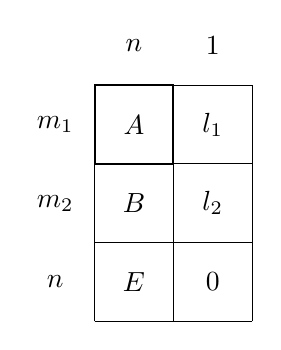
\begin{tikzpicture}[x=1cm, y=1cm]
      \draw(0, 2) -- (2, 2); % rows
      \draw(0, 1) -- (2, 1);
      \draw(0, 0) -- (2, 0);
      \draw(0,-1)-- (2,-1);
      %
      \draw(0,-1) -- (0,2); % cols
      \draw(1,-1) -- (1,2);
      \draw(2,-1) -- (2,2);
      %
      \draw[thick] (0,1) rectangle (1,2);     % top left cell
      %
      \draw(0.5,2.5) node{$n$};               %
      \draw(1.5,2.5) node{$1$};
      %
      \draw(-0.5,1.5) node{$m_1$};
      \draw(0.5,1.5) node{$A$};               % first row
      \draw(1.5,1.5) node{$l_1$};
      %%
      \draw(-.5,-0.5) node{$n$};
      \draw(-0.5,0.5) node{$m_2$};
      \draw(0.5,0.5) node{$B$};               % second row
      \draw(1.5,0.5) node{$l_2$};
      %
      \draw(0.5,-0.5) node{$E$};          % third row
      \draw(1.5,-0.5) node{$0$};
      %
    \end{tikzpicture} }}
    \quad{\raisebox{-0.35cm}{\ensuremath{\longrightarrow}}}\quad
    \vcenter{\hbox{
    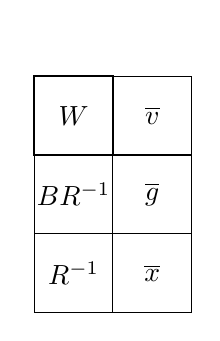
\begin{tikzpicture}[x=1cm, y=1cm]
      \draw(0,2) -- (2,2); % rows
      \draw(0,1) -- (2,1);
      \draw(0, 0) -- (2, 0);
      \draw(0,-1) -- (2,-1);
      %
      \draw(0,-1) -- (0,2); % cols
      \draw(1,-1) -- (1,2);
      \draw(2,-1) -- (2,2);
      %
      \draw[thick] (0,1) rectangle (1,2);     % top left cell
      %
      \draw(0.5,2.5) node{$~$};               %
      \draw(1.5,2.5) node{$~$};
      %
      \draw(0.5,1.5) node{$W$};               % first row
      \draw(1.5,1.5) node{$\overline{v}$};
      %%
      \draw(0.5,0.5) node{$BR^{-1}$};          % second row
      \draw(1.5,0.5) node{$\overline{g}$};
      %
      \draw(0.5,-0.5) node{$R^{-1}$};          % third row
      \draw(1.5,-0.5) node{$\overline{x}$};
      %
    \end{tikzpicture} }}%,
    %
\end{align*}
%

\vspace{1ex}
\noindent
kde jsme označili $\overline{g} = B \overline{x} + l_2$. Stejně jako
při užití \name{BESSELOVY} metody předpokládáme lineární nezávislost sloupců
matice A.  Tato podmínka ovšem není nutnou podmínkou pro řešitelnost
úlohy IC, jak ukazuje např \name{BAETSLE} [1]. Ortogonalizujme ve druhé etapě
podle schematu
%
\begin{align*}
  \tag{5.5}
    \vcenter{\hbox{
    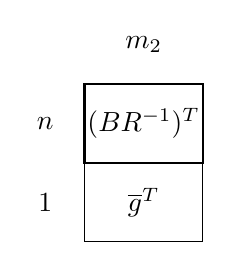
\begin{tikzpicture}[x=1cm, y=1cm]
      \draw(0, 0) -- (1.5, 0);
      %
      \draw(0,0) -- (0,2); % cols
      \draw(1.5,0) -- (1.5,2);
      %\draw(2,-1) -- (2,2);
      %
      \draw[thick] (0,1) rectangle (1.5,2);     % top left cell
      %
      \draw(0.75,2.5) node{$m_2$};               %
      %
      \draw(-0.5,1.5) node{$n$};
      \draw(0.75,1.5) node{$(BR^{-1})^T$};               % first row
      %%
      %\draw(-.5,-0.5) node{$n$};
      \draw(-0.5,0.5) node{$1$};
      \draw(0.75,0.5) node{$\overline{g}^T$};               % second row
      %\draw(1.5,0.5) node{$$};
      %
    \end{tikzpicture} }}
    \quad{\raisebox{-0.35cm}{\ensuremath{\longrightarrow}}}\quad
    \vcenter{\hbox{
    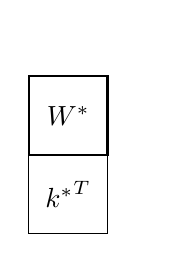
\begin{tikzpicture}[x=1cm, y=1cm]
      \draw(0,2) -- (1,2); % rows
      \draw(0,1) -- (1,1);
      \draw(0, 0) -- (1, 0);
      %
      \draw(0,0) -- (0,1); % cols
      \draw(1,0) -- (1,1);
      %
      \draw[thick] (0,1) rectangle (1,2);     % top left cell
      %
      \draw(0.5,2.5) node{$~$};               %
      \draw(1.5,2.5) node{$~$};
      %
      \draw(0.5,1.5) node{$W^*$};               % first row
      %
      \draw(0.5,0.5) node{${k^*}^T$};          % second row
      %
    \end{tikzpicture}}}%,
    %
\end{align*}
%

\noindent
Po delším odvození lze dokázat (poznámka 1 na str.~\pageref{XLVI}), že
pro hledané opravy $v$ a neznámé $x$ platí
%
\begin{align*}
  \tag{5.6}
  v = \overline{v} - WW^*k^*, \qquad x = \overline{x} - R^{-1}W^*k^*,
\end{align*}

\noindent
kde všechny potřebné veličiny byly získány dvojí ortogonalizací
podle (5.4) a (5.5). Přitom ze zřejmých důvodů předpokládáme při
druhé ortogonalizaci lineární nezávislost řádků matice~$B$.

Naznačená cesta je aplikovatelná i pro vyrovnání podmínkových
pozorování s neznámými, jak ukazujeme v poznámce 2 na
str.~\pageref{XLVIII}.  Přesto se však nezdá být dobrým základem pro
univerzální vyrovnávací metodu, zejména proto, že tříští ucelenost
algoritmu a může mít singulární průběh i u regulárních úloh (lineárně
závislé sloupce matice $A$).

Zkusíme proto užít jiného principu, který by umožnil řešit úlohy typu
IC a CU postupem co nejbližším postupu užívanému při vyrovnání
zprostředkujících nebo podmínkových pozorování.  Takovému požadavku
vyhovuje např. metoda navržená \name{H.H.SCHMIDEM} [33], [57], [25],
[43,str.525]. Základní myšlenka této metody spočívá
%
%
v tom, \orig{39}
že úlohy typu IC (resp. CU) řeší identickým způsobem
jako vyrovnání zprostředkujících (resp. podmínkových) pozorování,
ovšem za předpokladu, že váhy některých firgovaných veličin
nabývají extrémních hodnot. Přesněji:
%
\Xemph
{
   v případě IC se rovnice (5.2) pokládají za rovnice oprav s vahou
   rostoucí  nade všechny meze, v případě CU se neměřené neznámé $x$
   pokládají za opravy měřených veličin, jimž přísluší nulová váha.
}
%
Ověříme logiku takového
postupu, aniž bychom prováděli exaktní důkaz o jeho správnosti.
Přisoudíme-li při vyrovnání zprostředkujících pozorování
některé rovnici oprav relativně velkou váhu, pak předpokládáme, že
střední chyba odpovídající pozorované hodnoty je malá a
očekáváme, že vyrovnávací mechanismus přiřadí této hodnotě relativně
malou opravu. V aplikaci na IC budou tedy s rostoucí vahou
klesat absolutní hodnoty oprav uvažovaných na levé straně rovnic
(5.2). V limitním případě pak budou levé strany (5.2) anulovány.
Přisoudíme-li naopak při vyrovnání podmínkových pozorování
některým pozorovaným hodnotám relativně malou váhu, pak
připouštíme jejich relativně velkou nejistotu. V souladu s~tím má
vyrovnávací mechanismus "volnost" při určení odpovídajících oprav.
Aniž by byl prakticky vázán nějakou podmínkou omezující jejich
velikost, určí je tak, aby součet čtverců pouze zbývajících
oprav byl minimální při současném splnění podmínkových rovnic. S
klesající vahou budou tak opravy dostávat charakter neměřených
neznámých.

Při aplikaci \name{SCHMIDOVY} metody nemůžeme ovšem volit extrémní
hodnoty vah, ale pouze hodnoty relativně velké nebo malé
vzhledem k ostatním vahám (v našich úvahách jednotkovým). Okamžitě
tak narážíme na otázku, jakých hodnot užít při praktickém
výpočtu. Pro ilustraci dalších úvah uvedeme výsledky jednoho
numerického testu.

Malá zkušební úloha typu CU s maticemi
$A^T (8\times14)$, $B^T (8\times4)$,
vzatá z oboru vyrovnání prostorových sítí, byla počítána v
několika alternativách. Obvyklým postupem podle známých vzorců
platných pro úlohy kategorie CU byly především určeny etalonní
výsledky. S těmito výsledky byly potom porovnány výsledky získané
vyrovnáním téže úlohy podle podmínkových pozorování, kde čtyři
%
neměřené \orig{40} neznámé byly nahrazeny opravami s vahou
$\varepsilon$ příslušných fiktivních pozorovaných hodnot měněnou v
intervalu $<\!10^{-6},  10^4\!>$. Výpočet byl realizován na počítači ODRA 1003
(mantisa 31 bitů) podle programu MNČ-ODRA-VM [21], založeného na
inverzi matice soustavy normálních rovnic. Zjištěné diference oprav
resp. neznámých byly potom podle (4.9) vzaty za základ odhadu počtu
platných cifer $p_v$ resp. $p_x$ výsledků vyrovnání podle podmínkových
pozorování. Průběh charakteristik přesnosti $p_v$ a $p_x$ závislosti
na volbě $\varepsilon$ ukazuje obr. 5.1.

\begin{center}
\includegraphics[width=0.5\textwidth]{obr_5.1.png}\\
Obr. 5.1
\end{center}

\noindent
Z obrázku vidíme, že počet platných cifer výsledků s klesající
vahou nejprve stoupá. To odpovídá naší představě, podle níž
očekáváme, že s klesající vahou se bude postupně stírat rozdíl mezi
fiktivní opravou a neměřenou neznámou.
\Xemph{Od určité hodnoty váhy}
(v našem příkladě kolem $10^0$) \Xemph{počínaje}, však naopak
\Xemph{pozorujeme výrazný pokles přesnosti}.
Při užití váhy menší než přibližně $10^{-7}$ dostáváme dokonce
prakticky bezcenné výsledky. Ukážeme na zákonitost tohoto jevu.


Nechť $[A^T B^T]$ je matice soustavy podmínkových rovnic. Matice $A^T$
nechť odpovídá opravám s jednotkovými vahami, matice $B^T$ pak opravám
s vahami $\varepsilon$. Matice soustavy normálních rovnic je potom
%
\begin{align*}
\tag{5.7}
        N = (A^TA + \varepsilon^{-1}B^TB).
\end{align*} \orig{41}
%
Předpokládejme nyní, že jsme váhu $\varepsilon$ volili řádově menší
než jedna. Pokud prvky matic $A$ a $B$ byly řádově stejné, pak zřejmě
druhý sčítanec ve (5.7) bude řádově větší než sčítanec první, který se
tak na celkovém součtu uplatní tím méně, čím menší bude
$\varepsilon$. Vzhledem k tomu, že počítač pracuje s konečným počtem
cifer, nastane pro určitou hodnotu č dokonce situace, kdy
%
\begin{align*}
\tag{5.8}
        \varepsilon N = B^TB.
\end{align*}
%
Hodnost matice $B^T(n \times m_2)$ může být nejvýše rovna $m_2$.  Podle
[37, str. 115] nemůže být hodnost $h$ matice $\varepsilon N(n \times
n)$ větší než $m_2$.  Protože je ale zpravidla ve všech praktických
případech $n > m_2$, bude $h \le m_2 < n$.  Matice $\varepsilon N$
bude tedy singulární a pokus o numerické řešení odpovídající soustavy
selže. V našem příkladě byly prvky matice $A$ řádu $10^0$ a prvky
matice $B$ řádu $10^2$. Uvážíme-li současně, že počítač ODRA pracuje
přibližně s devíticifernými mantisami, pak můžeme očekávat, že matice
$N$ bude prakticky singulární již pro hodnoty $\varepsilon \approx
10^{-5}$. Ke stejnému závěru jsme došli analýzou výsledků experimentu.

%
%
\Xemph{Souhrnně můžeme konstatovat, že pokles přesnosti řešení je
důsledkem numerické nestability metody, vyvolané špatnou podmíněností
matice soustavy normálních rovnic}.\footnote%
{
V jiné souvislosti komentuje analogickou situaci \name{MAZMIŠVILI}
[28, str. 206] takto:~
\selectlanguage{russian}%
``... если началъные уравнения cбалансированы по весам
недостаточно, то надежность решения системы нормалъных
уравнений остается под сомнением.''
\selectlanguage{czech}%
}
%
%\includegraphics{mazmisvili-citace.png}
%
% Karel Vach
%
%``... pokud nejsou počáteční rovnice dostatečně přesně váhově
% vyvážené, potom spolehlivost řešení soustavy normálních rovnic je
% na pochybách.''
%
% AČ
%
% ``... pokud nejsou počáteční rovnice dostatečně vyvážené, pak se
% spolehlivost řešení soustavy normálních rovnic stává pochybnou.''
%


Je pravděpodobné, že nalezení
optimální hodnoty váhy $\varepsilon$, při níž je možno dosáhnout
maximální přesnosti řešení, by v obecném případě bylo dosti
obtížné. Kromě toho může být i maximálně dosažitelná přesnost poměrně
nízká, jak se ostatně ukázalo i v uvedeném příkladě.

Prozatím jsme zkoumali spojení \name{SCHMIDOVA} principu s klasickým
vyrovnávacím postupem, vycházejícím ze řešení soustavy
normálních rovnic. Zkusme ještě kombinovat stejný princip s~metodou
ortogonalizační. Závěry odvozené pro řešení špatně podmíněných
úloh v kap. 4 nás k takovému postupu opravňují. Nejprve opět
uvedeme výsledky numerického experimentu se stejnou zkušební
úlohou. \orig{42} Obr. 5.2 znázorňuje průběh charakteristik přesnosti $p_v$ a
$p_x$, výsledků, získaných užitím zobecněného ortogonalizačního
algoritmu v aplikaci na vyrovnání podmínkových pozorování (odst.
3.2). Váha $\varepsilon$ byla tentokrát volena v intervalu
$<\!10^{-10}, 10^4\!>$.


\begin{center}
\includegraphics[width=0.75\textwidth]{obr_5.2.png}\\
Obr. 5.2
\end{center}

\noindent
Z obr. 5.2 je především patrno, že ortogonalizační metoda i zde dává
přesnější výsledky než přechod na řešení normálních rovnic. Dále
zjišťujeme zejímavou skutečnost, že přesnost v~určení oprav je jiná
(vyšší) než přesnost určení neznámých.  Z obr. 5.2 můžeme kromě toho
usoudit, že i zde zůstává optimální volba váhy problémem. Jinými
slovy: \Xemph{špatná podmíněnost úlohy vyvolaná příliš malou vahou
$\varepsilon$ může mít i při standardním užití ortogonalizace
nepříznivý vliv na přesnost výsledků.}


Zkoumejme nyní podrobněji projevy špatné podmíněnosti úlohy
v průběhu jejího řešení ortogonalizačním algoritmem. V kap. 3
\orig{43}
jsme ukázali, že zavedeme-li do vyrovnání obecné hodnoty vah,
pak je třeba odmocninami z vah násobit resp. dělit
odpovídající řádky ve schematech (3.19) resp. (3.37). Základními
submaticemi při řešení úloh IC resp. CU podle uvedených schemat
jsou potom matice
%
\begin{align*}
\tag{5.9}
    \vcenter{\hbox{
    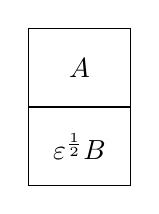
\begin{tikzpicture}[x=1cm, y=1cm]
      \def\dx{1.3cm};
      \def\dy{1cm};
      %
      \draw (0, 1*\dy) rectangle (\dx, 2*\dy);   % top rectangle
      \draw(0.5*\dx,1.5*\dy) node{$A$};
      %
      \draw (0, 0*\dy) rectangle (\dx, 1*\dy);   % bottom rectangle
      \draw(0.5*\dx,0.5*\dy) node{$\varepsilon^{1\over2}B$};
      %
    \end{tikzpicture} }}
    %
    \quad\textrm{resp.}\quad
    %
    \vcenter{\hbox{
    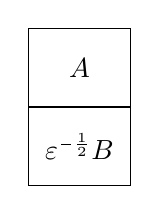
\begin{tikzpicture}[x=1cm, y=1cm]
      \def\dx{1.3cm};
      \def\dy{1cm};
      %
      \draw (0, 1*\dy) rectangle (\dx, 2*\dy);   % top rectangle
      \draw(0.5*\dx,1.5*\dy) node{$A$};
      %
      \draw (0, 0*\dy) rectangle (\dx, 1*\dy);   % bottom rectangle
      \draw(0.5*\dx,0.5*\dy) node{$\varepsilon^{{~\over~}{1\over2}}B$};
      %
    \end{tikzpicture} }},
    %
\end{align*}
%
přičemž v prvním případě studujeme extrémní případ
$\varepsilon\rightarrow\infty$ a ve druhém limitu
$\varepsilon\rightarrow0$. Z~numerického hlediska jsou oba procesy
identické, stačí tedy sledovat průběh ortogonalizace matice
%
% V původním rukopisu není jasné, jestli matice A v (5.10) a dále
% má být indexována s velkým O, nulou nebo malým o (třeba ve fontu \tt).
% Patrně byl míněn index s písmenem O velkým/malým jako ortogonalizovaná.
%
% Nakonec jsem se ale rozhodnul pro index 0 (nula), protože malé o
% mi přišlo vzhledově nepřirozené (ať už \tt nebo \rm).
%
% Pro indexování matic A jsem zavedl macro \Amat, použití
% např.  \Amat{}, \Amat{0} nebo \Amat{01}.
%
% Je otázka zda nedefinovat obdobně i další matice, např. \Bmat,
%
\begin{align*}
\tag{5.10}
   %{\raisebox{-0.22cm}{\ensuremath{A_O = \,}}}
    {\raisebox{-0.22cm}{ \Amat{0} = }}
    \vcenter{\hbox{
    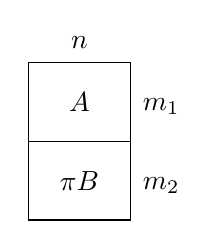
\begin{tikzpicture}[x=1cm, y=1cm]
      \def\dx{1.3cm};
      \def\dy{1cm};
      %
      \draw (0, 1*\dy) rectangle (\dx, 2*\dy);   % top rectangle
      \draw(0.5*\dx,1.5*\dy) node{$A$};
      %
      \draw (0, 0*\dy) rectangle (\dx, 1*\dy);   % bottom rectangle
      \draw(0.5*\dx,0.5*\dy) node{$\pi B$};
      %
      \draw(0.5*\dx,2.25*\dy) node{$n$};
      \draw(1.3*\dx,1.44*\dy) node{$m_1$};
      \draw(1.3*\dx,0.44*\dy) node{$m_2$};
      %
    \end{tikzpicture} }}
    %
\end{align*}
%
kde číselný parametr $\pi$ roste nade všechny meze.  Předpokládejme
pro jednoduchost, že prvky matic A a B jsou řádu \Ocal{10^0}.  Dále
nechť $\delta$ představuje relativní zaokrouhlovací chybu užitého
počítače.
%
\footnote
{
Zaokrouhlovací chyba $\delta$ je definována [15, str. 110] výrazem
$0.5\beta^{1-t}$, kde $\beta$ je základ číselné soustavy a $t$ je
počet cifer mantisy čísla, vyjádřeného ve tvaru s pohyblivou řádovou
čárkou. V případě počítače ODRA je $\delta=5\times10^{-10}$;
zaokrouhlovací chyba počítače ELLIOTT 503 je $\delta =
2\times10^{-9}$.%
}
%

Matici \Amat{0} rozdělíme na submatice
%
\begin{align*}
\tag{5.11}
\Amat{0} =
%
\vcenter{\hbox{
   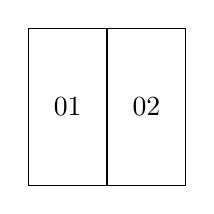
\begin{tikzpicture}[x=1cm, y=1cm]
   \def\dx{1cm};
   \def\dy{1cm};
   \draw (0,  -\dy) rectangle (\dx, \dy);   % left rectangle
   \draw(0.5*\dx,0) node{\Amat{01}};
   \draw (\dx, -\dy) rectangle (2*\dx, \dy);   % right rectangle
   \draw(1.5*\dx,0) node{\Amat{02}};
   \end{tikzpicture} }}
   =
\raisebox{-6.53ex}{\hbox{
   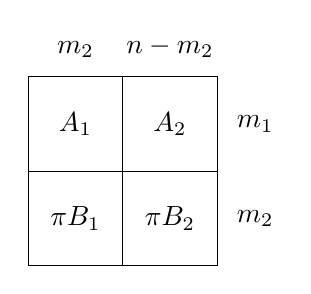
\begin{tikzpicture}[x=1cm, y=1cm]
   \def\dx{1.2cm};
   \def\dy{1.2cm};
   \draw (0,  -\dy) rectangle (\dx, \dy);   % left rectangle
   \draw (\dx, -\dy) rectangle (2*\dx, \dy);   % right rectangle
   \draw (0,0) -- (2*\dx,0);
   \node[label=above:{$m_2$}] at (0.5*\dx,\dy) {};
   \node[label=above:{$n-m_2$}] at (1.5*\dx,\dy) {};
   \node[label=right:{$m_1$}] at (2*\dx,0.5*\dy) {};
   \node[label=right:{$m_2$}] at (2*\dx,-0.5*\dy) {};
   \draw(0.5*\dx,0.5*\dy) node{$A_1$};
   \draw(1.5*\dx,0.5*\dy) node{$A_2$};
   \draw(0.5*\dx,-0.5*\dy) node{$\pi B_1$};
   \draw(1.5*\dx,-0.5*\dy) node{$\pi B_2$};
   \end{tikzpicture} }}
%
\end{align*}
%

\noindent
O čtvercové \orig{44} matici $B_1 (m_2\times m_2)$ předpokládáme, že
je regulární.  Takový předpoklad je zřejmě možný: matice B(m x n) má
lineárně nezávislé řádky, musí mít tedy i $m_2$ lineárně nezávislých
sloupců. Vhodným uspořádáním sloupců matice \Amat{0} je pak vždy možno
docílit toho, aby sloupce matice $B_1$ byly lineárně nezávislé.
Probereme nyní odděleně ortogonalizaci každé ze submatic \Amat{01} a
\Amat{02}. Matici vzniklou ortogonalizací \Amat{0} označíme

\begin{align*}
\tag{5.12}
W =
%
\vcenter{\hbox{
   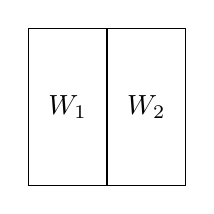
\begin{tikzpicture}[x=1cm, y=1cm]
   \def\dx{1cm};
   \def\dy{1cm};
   \draw (0,  -\dy) rectangle (\dx, \dy);   % left rectangle
   \draw(0.5*\dx,0) node{$W_1$};
   \draw (\dx, -\dy) rectangle (2*\dx, \dy);   % right rectangle
   \draw(1.5*\dx,0) node{$W_2$};
   \end{tikzpicture} }}
   =
\vcenter{\hbox{
   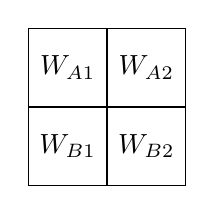
\begin{tikzpicture}[x=1cm, y=1cm]
   \def\dx{1.cm};
   \def\dy{1.cm};
   \draw (0,  -\dy) rectangle (\dx, \dy);   % left rectangle
   \draw (\dx, -\dy) rectangle (2*\dx, \dy);   % right rectangle
   \draw (0,0) -- (2*\dx,0);
   \draw(0.5*\dx,0.5*\dy) node{$W_{A1}$};
   \draw(1.5*\dx,0.5*\dy) node{$W_{A2}$};
   \draw(0.5*\dx,-0.5*\dy) node{$W_{B1}$};
   \draw(1.5*\dx,-0.5*\dy) node{$W_{B2}$};
   \end{tikzpicture} }}
%
\end{align*}



Aplikujeme-li ortogonalizační vzorce např. (2.1) na zpracování
matice \Amat{01} zjistíme především, že pro každou hodnotu $\delta$
bude existovat určitá hodnota $\pi$, od níž počínaje proběhne
ortogonalizace ve spodní části matice $A_{O1}$ nezávisle na matici
$A_1$.  Matice $W_{B1}$ bude tedy v limitě totožná s maticí, kterou
bychom dostali samostatnou ortogonalizací matice $B_1$. Snadno lze
dokázat, že matice $W_{B1}$ je ortogonální. Prvky matice $A_1$, se při
dostatečně velké hodnotě $\pi$ nepodílejí na tvorbě skalárních součinů
ani normalizačních faktorů ve (2.1$_2$) a (2.1$_3$). Probíhá tedy
zpracování matice $A_1$ analogicky jako ortogonalizace submatice $A_3$
ve (2.16).  Podle (2.20) platí $W_{A1} = A_1R^{-1}$, při $\pi B_1 =
W_{B1}R$, takže $W_{A1} = \pi^{-1}A_1B_1^{-1}W_{B1}$.  Při dobré
podmíněnosti matice $B_1$ můžeme potom očekávat, že prvky matice
$W_{A1}$ budou řádu \Ocal{\pi^{-1}}.
%
Stejně jako zpracování matice $\pi\Bmat{1}$ není za uvedených
předpokladů ani zpracování matice \Amat{1} provázeno známkami
numerické nestability.

Obraťme se nyní k ortogonalizaci $\Amat{02} \rightarrow \Wmat{2}$.
Ortogonalizací některého sloupce
%
$a_2 = \begin{bmatrix} a_{\Amat{2}} \\ b_{\Bmat{2}}\end{bmatrix}$
%
matice \Amat{02} ke sloupcům matice \Wmat{1} např. podle vzorce
($2.1_2$) nechť vznikne vektor, který označíme
%
$\widetilde w_2 =
\begin{bmatrix} \widetilde w_{\Amat{2}} \\
                \widetilde w_{\Bmat{2}}\end{bmatrix}$.
%
Připomeňme, že prvky matice \Wmat{A1} resp. \Bmat{B1} jsou přibližně
řádu \Ocal{\pi^{-1}} resp. \Ocal{10^0} a prvky vektoru
$a_{\Amat{2}}$ resp. $a_{\Bmat{2}}$ řádu přibližně \Ocal{10^0}
resp. \Ocal{\pi}, schematicky\orig{45}
%
\begin{align*}
\tag{5.13}
    \vcenter{\hbox{
    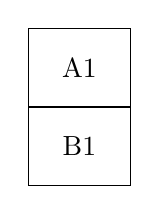
\begin{tikzpicture}[x=1cm, y=1cm]
      \def\dx{1.3cm};
      \def\dy{1cm};
      %
      \draw (0, 1*\dy) rectangle (\dx, 2*\dy);   % top rectangle
      \draw(0.5*\dx,1.5*\dy) node{\Wmat{A1}};
      %
      \draw (0, 0*\dy) rectangle (\dx, 1*\dy);   % bottom rectangle
      \draw(0.5*\dx,0.5*\dy) node{\Wmat{B1}};
      %
    \end{tikzpicture} }}
    %
    \quad\sim\quad %-------------------------------------
    %
    \vcenter{\hbox{
    \begin{tikzpicture}[x=1cm, y=1cm]
      \def\dx{1.3cm};
      \def\dy{1cm};
      %
      \draw (0, 1*\dy) rectangle (\dx, 2*\dy);   % top rectangle
      \draw(0.5*\dx,1.5*\dy) node{\Ocal{\pi^{-1}}};
      %
      \draw (0, 0*\dy) rectangle (\dx, 1*\dy);   % bottom rectangle
      \draw(0.5*\dx,0.5*\dy) node{\Ocal{10^0}};
      %
    \end{tikzpicture} }} \Punc{,}
%%%%%%%%%%%%%%
    \qquad\quad
    \vcenter{\hbox{
    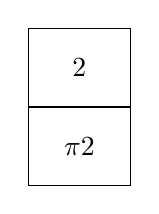
\begin{tikzpicture}[x=1cm, y=1cm]
      \def\dx{1.3cm};
      \def\dy{1cm};
      %
      \draw (0, 1*\dy) rectangle (\dx, 2*\dy);   % top rectangle
      \draw(0.5*\dx,1.5*\dy) node{\Amat{2}};
      %
      \draw (0, 0*\dy) rectangle (\dx, 1*\dy);   % bottom rectangle
      \draw(0.5*\dx,0.5*\dy) node{$\pi\Bmat{2}$};
      %
    \end{tikzpicture} }}
    %
    \quad\sim\quad %----------------------------------------
    %
    \vcenter{\hbox{
    \begin{tikzpicture}[x=1cm, y=1cm]
      \def\dx{1.3cm};
      \def\dy{1cm};
      %
      \draw (0, 1*\dy) rectangle (\dx, 2*\dy);   % top rectangle
      \draw(0.5*\dx,1.5*\dy) node{\Ocal{10^0}};
      %
      \draw (0, 0*\dy) rectangle (\dx, 1*\dy);   % bottom rectangle
      \draw(0.5*\dx,0.5*\dy) node{\Ocal{\pi}};
      %
    \end{tikzpicture} }} \Punc{.}
%
\end{align*}

%
Kdybychom analogicky jako prve izolovaně ortogonalizovali pouze
vektor $b_{\Bmat{2}}$ k matici \Wmat{B1} pak by zřejmě vektor
$\widetilde w_{\Bmat{2}}$ byl nulový.
%
Sloupce matice $\pi\Bmat{1}$ tvoří totiž bázi $m_2$-rozměrného
prostoru a všechny další vektory tohoto prostoru, tedy i vektor
$b_{\Bmat{B2}}$, mohou být vyjádřeny jako jejich lineární kombinace.
%
Vektor $b_{\Bmat{2}}$ je tak lineárně závislý na sloupcích matice
$\pi\Bmat{1}$ a podle našeho konstatování v kap. 2 bude odpovídající
sloupec $\widetilde w_{\Bmat{2}}$ nulový.
%
Izolovaná ortogonalizace sloupce $b_{\Bmat{2}}$ odpovídá limitnímu
případu jeho zpracování při ortogonalizaci celého sloupce $a_2$,
pro $\pi \rightarrow \infty$.
%
Je-li $\pi$ konečné, pak prvky vektoru  $\widetilde w_{\Bmat{2}}$
nebudou nulové, ale budou řádu \Ocal{\pi}.
O prvcích vektoru $\widetilde w_{\Bmat{2}}$ lze podrobnějším
rozborem prokázat, že za určitých předpokladů budou řádu \Ocal{10^0}.
Při numerickém výpočtu dostáváme složky vektoru
$\widetilde w_{\Bmat{2}}$ slučováním čísel
řádu přibližně \Ocal{10^0}, jejich chyba bude tedy řádu
\Ocal{\delta}.
%
Složky vektoru $\widetilde w_{\Bmat{2}}$ dostáváme slučováním čísel
řádu přibližně \Ocal{\pi}, takže odpovídající řád chyby je
\Ocal{\pi\delta}.
%
Relativní chyba prvků vektoru $\widetilde w_{\Bmat{2}}$
je tedy přibližně řádu \Ocal{\pi\delta} a je proto
dostatečně malá.
%
Naproti tomu relativní chyba prvků vektoru $\widetilde w_{\Bmat{2}}$
je již pro $\pi > \delta^{-{1\over2}}$ řádu \Ocal{10^0}, čili
od
%
\Xemph{určitého $\pi$ počínaje
nebudou mít prvky vektoru $\widetilde w_{\Bmat{2}}$
žádnou platnou cifru.}
%
Uvážíme-li způsob výpočtu oprav při vyrovnání podmínkových pozorování
ortogonalizační metodou (odst. 3.2), snadno najdeme vysvětlení, proč
byly v našem příkladě neměřené neznámé nalezeny s větší nejistotou než
opravy.


Označme $\varphi$ vektor chyby vektoru $\widetilde w_{\Bmat{2}}$.
Rozložme $\varphi$ na součet dvou vektorů
%
\begin{align*}
\tag{5.14}
\varphi = \varphi_1 + \varphi_2 =
\begin{bmatrix} 0 \\ \varphi_{11} \end{bmatrix} +
\begin{bmatrix} \varphi_{22} \\ 0 \end{bmatrix}
\quad\begin{matrix} m_1 \\ m_2 \end{matrix} \Punc{.}
\end{align*}
%
\orig{46}
%
Pro dostatečně velká $\pi$ lze dokázat, že vektor $\varphi_1$,
prakticky leží v prostoru vytvářeném sloupci matice \Wmat{1}, vektor
$\varphi_2$ je naopak ortogonální ke všem těmto sloupcům. Skutečně,
vektor $\varphi_1$ může být s dostatečnou přesností vyjádřen jako
lineární kombinace sloupců matice \Wmat{1}. Na druhé straně skalární
součiny vektoru $\varphi_2$, se sloupci matice \Wmat{1} jsou řádu
\Ocal{\delta\pi^{-1}}, v limitě neomezeně klesajícího.


Došli jsme tedy k závěru, že \Xemph{numerický výpočet je při spojení
ortogonalizace se \name{SCHMIDOVÝM} principem extremálních vah
znehodnocován především ortogonálními projekcemi $\varphi_1$ celkových
chyb $\varphi$ vektorů $\widetilde w_2$ na podprostor, tvořený sloupci
matice \Wmat{1}}. V další kapitole ukážeme způsob, kterým bude možno
tyto složky chyb eliminovat a tak dále zvýšit numerickou stabilitu
metody.


\Pozn{1} \label{XLVI} Dokážeme platnost vzorců (5.6) pro určení oprav
a neznámých v úloze typu IC metodou dvojí ortogonalizace podle
(5.4) a (5.5). Užijeme-li rozkladu (2.10) a vztahu (2.7),
můžeme soustavu normálních rovnic, na něž vede klasický způsob
přímého řešení úlohy [49,str.210], psát ve tvaru
%
\begin{align*}
\tag{5.15}      R^TRx& + B^Tk + R^TW^Tl_1 = 0\\
\tag{5.16}      Bx&           + l_2      = 0 \Punc{,}
\end{align*}
%
kde $k$ je vektor korelát. Pokud jsou sloupce matice \Amat{} lineárně
nezávislé, můžeme z (5.15) vyjádřit vektor $x$ a dosadit do (5.16),
Dostaneme
%
\begin{align*}
\tag{5.17}     &x = -(R^TR)^{-1}(B^Tk + R^TW^Tl_1)\\
\tag{5.18}     &B(R^TR)^{-1} (B^Tk + R^TW^Tl_1) - l_2 = 0 \Punc{.}
\end{align*}
%
Neznámé $\overline{x}$ a opravy $\overline{v}$, odpovídající vyrovnání
(5.1) podle zprostředkujících pozorování při zanedbání podmínek
(5.2), jsou s užitím (3.7) a (3.8) dány vzorci
%
\begin{align*}
\tag{5.19}      &\overline{x} = -(R^TR)^{-1}R^TW^Tl_1\\
\tag{5.20}      &\overline{v} = WR\overline{x}l_1 \Punc{.}
\end{align*}
%
Po dosazení \orig{47} z (5.19) do (5.17) a (5.18) bude
\begin{align*}
\tag{5.21}     &x = \overline{x} - (R^TR)^{-1}B^Tk\\
\tag{5.22}     &(R^TR)^{-1}B^Tk - (B\overline{x} + l_2) = 0 \Punc{.}
\end{align*}
%
Uvažujme nyní soustavu podmínkových rovnic
%
\begin{align*}
\tag{5.23}     BR^{-1}w - (B\overline{x} + l_2) = 0 \Punc{.}
\end{align*}
%
S opravami $w$. Předpokládáme, že řádky matice soustavy (5.23) jsou
lineárně nezávislé. Vycházejíce ze (3.23), snadno se přesvědčíme o
tom, že řešení soustávy (5.23) podle metody nejmenších čtverců vede k
normálním rovnicím (5.22), takže v souladu s (325) platí
%
\begin{align*}
               w = R^{-T}B^{T}k \Punc{.}
\end{align*}
%
Dosadíme-li z (5.24) do (5.21) dostaneme
\begin{align*}
\tag{5.25}     x = \overline{x} - R^{-1}w \Punc{.}
\end{align*}
%
Dále je
%
\begin{align*}
\tag{5.26}     v = Ax + l_1 = WRx + l_1 - WR\overline{x} - Ww + l_1
                 = \overline{v} - Ww \Punc{.}
\end{align*}
%
Opravy $w$ můžeme podle (3.29) vyjádřit vzorcem
%
\begin{align*}
\tag{5.27}        w = W^*R^{*{-T}}\overline{g} \Punc{,}
\end{align*}
%
kde $W^*$ a $R^*$ jsou součinitelé v rozkladu (2.10) matice
transponované k matici soustavy podmínkových rovnic (5.23)
%
\begin{align*}
\tag{5.28}       (BR^{-1})^T = W^*R^*
\end{align*}
%
a vektor
%
\begin{align*}
\tag{5.29}       \overline{g} = B \overline{x}  + l_2
\end{align*}
%
je až na znaménko roven vektoru absolutních členů rovnic (5.23). Podle
(3.35) dostaneme ortogonalizací (5.5) matici $W^*$ a vektor
%
\begin{align*}
\tag{5.30}       k^{*^T} = (~\overline{g}~)^T R^{*^{-1}} \Punc{,}
\end{align*}
%
takže \orig{48} po dosazení z (5.30) do (5.27) je
%
\begin{align*}
\tag{5.31}       w = W^*k^* \Punc{.}
\end{align*}
%
S takto vyjádřeným vektorem oprav w dostávají rovnice (5.25)
a (5.26) konečnou formu
%
\begin{align*}
\tag{5.32}       x &= \overline{x} - R^{-1} W^*k^* \Punc{,} \\
                 v &= \overline{v} - WW^*k^*      \Punc{.}
\end{align*}
%
%
Vzorce (5.6) tedy platí.



\Pozn{2} \label{XLVIII} Odvodíme postup pro vyrovnání podmínkových
pozorování s neznámými metodou dvojí ortogonalizace. Soustavu
podmínkových rovnic (5.3) můžeme s užitím rozkladu
$A = WR$ psát ve tvaru
%
\begin{align*}
\tag{5.33}     W^Tv + R^{-T}B^Tx + R^{-T}u^T = 0 \Punc{.}
\end{align*}
%
Předpokládáme pro jednoduchost, že matice $A^T$ má lineárně nezávislé
řádky a matice $B^T$ lineárně nezávislé sloupce. Protože platí (2.7),
je možno ukázat [21, str.17], že rovnicím (5.33) odpovídá soustava
normálních rovnic
%
\begin{align*}
\tag{5.34}    BR^{-1}R^TB^Tx + BR^{-1}R^{-T}u^T - 0
\end{align*}
%
a opravy
%
\begin{align*}
\tag{5.35}    v = -W(R^{-T}B^Tx + R^{-T}u^T) \Punc{.}
\end{align*}
%
Podle (3.3) vede ke stejným normálním rovnicím (5.34) i řešení
soustavy rovnic oprav
%
\begin{align*}
\tag{5.36}   w = R^{-T}B^Tx + R^{-T}u^T .
\end{align*}
%
Můžeme tedy neznámé $x$ najít vyrovnáním náhradní úlohy (5.36)
podle zprostředkujících pozorování. Hledané opravy $v$ určuje po
dosazení z (5.36) do (5.35) rovnice
%
\begin{align*}
\tag{5.37}      v = -WW \Punc{.}
\end{align*}
%
Neznámé $x$, stejně jako veličiny $W$ a $w$ , potřebné k výpočtu oprav
$v$ podle (5.37), lze najít dvěma zobecněnými
ortogonalizacemi \orig{49}
%
\begin{align*}
\tag{5.38}
 \vcenter{\hbox{
     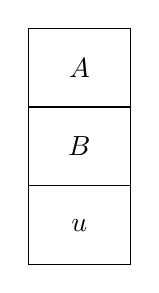
\begin{tikzpicture}[x=1cm, y=1cm]
      \def\dx{1.3cm};
      \def\dy{1cm};
      %
      \draw (0, 2*\dy) rectangle (\dx, 3*\dy);   % top rectangle
      \draw(0.5*\dx,2.5*\dy) node{$A$};
      %
      \draw (0, 1*\dy) rectangle (\dx, 2*\dy);   % middle rectangle
      \draw(0.5*\dx,1.5*\dy) node{$B$};
      %
      \draw (0, 0*\dy) rectangle (\dx, 1*\dy);   % bottom rectangle
      \draw(0.5*\dx,0.5*\dy) node{$u$};
      %
    \end{tikzpicture}}}
    \quad\longrightarrow\quad
 \vcenter{\hbox{
     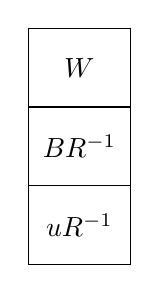
\begin{tikzpicture}[x=1cm, y=1cm]
      \def\dx{1.3cm};
      \def\dy{1cm};
      %
      \draw (0, 2*\dy) rectangle (\dx, 3*\dy);   % top rectangle
      \draw(0.5*\dx,2.5*\dy) node{$W$};
      %
      \draw (0, 1*\dy) rectangle (\dx, 2*\dy);   % middle rectangle
      \draw(0.5*\dx,1.5*\dy) node{$BR^{-1}$};
      %
      \draw (0, 0*\dy) rectangle (\dx, 1*\dy);   % bottom rectangle
      \draw(0.5*\dx,0.5*\dy) node{$uR^{-1}$};
      %
    \end{tikzpicture}}}
    %
    \quad\quad\quad\quad
    %
     \vcenter{\hbox{
     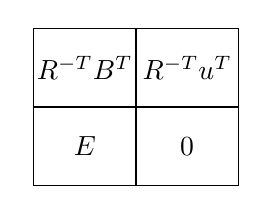
\begin{tikzpicture}[x=1cm, y=1cm]
      \def\dx{1.3cm};
      \def\dy{1cm};
      %
      \draw (0, 1*\dy) rectangle (\dx, 2*\dy);   % top left
      \draw(0.5*\dx,1.5*\dy) node{$R^{-T}B^T$};
      \draw (1*\dx, 1*\dy) rectangle (2*\dx, 2*\dy);   % top right
      \draw(1.5*\dx,1.5*\dy) node{$R^{-T}u^T$};
      %%
      \draw (0, 0*\dy) rectangle (\dx, 1*\dy);         % bottom left
      \draw(0.5*\dx,0.5*\dy) node{$E$};
      \draw (1*\dx, 0*\dy) rectangle (2*\dx, 1*\dy);   % bottom right
      \draw(1.5*\dx,0.5*\dy) node{$0$};
      %
    \end{tikzpicture}}}
    %
    \quad\longrightarrow\quad
    %
     \vcenter{\hbox{
     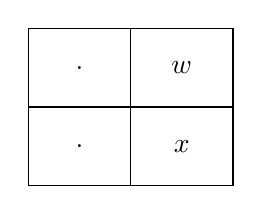
\begin{tikzpicture}[x=1cm, y=1cm]
      \def\dx{1.3cm};
      \def\dy{1cm};
      %
      \draw (0, 1*\dy) rectangle (\dx, 2*\dy);         % top left
      \draw(0.5*\dx,1.5*\dy) node{$.$};
      \draw (1*\dx, 1*\dy) rectangle (2*\dx, 2*\dy);   % top right
      \draw(1.5*\dx,1.5*\dy) node{$w$};
      %%
      \draw (0, 0*\dy) rectangle (\dx, 1*\dy);         % bottom left
      \draw(0.5*\dx,0.5*\dy) node{$.$};
      \draw (1*\dx, 0*\dy) rectangle (2*\dx, 1*\dy);   % bottom right
      \draw(1.5*\dx,0.5*\dy) node{$x$};
      %
    \end{tikzpicture}}}
%
 \Punc{.}
\end{align*}
%
První ortogonalizace vychází ze (3.35), druhá ze (3.18). Stejně jako
při vyrovnání úloh typu IC jsou i zde při druhé ortogonalizaci
zpracovávány submatice získané první ortogonalizací.
